\procTitle{Инженерные уроки (разработка демонстрационных установок)}
\procAuthor{Лейбович~Е.\,О., Ус~Я.\,М., Магомедов~М.}
\procEmail{evgeniiamgdn@gmail.com, yanina4444@icloud.com, 05ru9479@gmail.com}
\procOrganization{СВГУ} \procCity{Магадан}

\makeProcTitle
\index{l@Лейбович~Е.\,О.}
\index{y@Ус~Я.\,М.}
\index{m@Магомедов~М.}

Количество абитуриентов, поступающих на технические специальности, в последние годы продолжает снижаться. Соответственно, отрасли инженерной деятельности испытывают недостаток новых кадров. В то же время на основании проведённых Московской школой управления <<Сколково>> и Агентством стратегических инициатив исследований до 2030\,г. предполагается появление 136 новых профессий, среди которых: архитектор энергонулевых домов, проектировщик дирижаблей, архитектор территорий, урбанист-эколог, инженер роботизированных систем и многие другие [1].

Таким образом, вопрос о повышении интереса современной молодёжи к инженерному направлению продолжает оставаться актуальным. В ближайшем и более далёком будущем однозначно останутся востребованы специалисты в области естественных наук и инженерии. А это значит, что надо заинтересовать детей уже младшего школьного возраста в изучении физики, химии, математики и астрономии.

В Северо-Восточном государственном университете на протяжении последних трёх лет реализуется проект научно-познавательной площадки <<Эврика>>, целью которого является организация работы со школьниками по вовлечению их в процесс активного познания мира. Студентами разработаны и проведены в школах города и области мероприятия, которые наглядными экспериментами знакомили школьников с основами естественных наук (в частности, физики). В ходе мероприятий детям позволяется самостоятельно проводить несложные и безопасные эксперименты.

Особенностью нового элемента нашей площадки является инженерное направление. Сейчас мы предлагаем для проведения познавательных мероприятий три новые установки, разработанные студентами политехнического института. Эти установки демонстрируют законы физики, лежащие в основе работы многих механизмов.

Основной нашей целевой аудиторией являются представители поколения Z. Но многие из участников наших больших мероприятий ещё недостаточно самостоятельны, и поэтому сопровождаются взрослыми~--- родственниками, учителями и т.\,п. Это могут быть как представители поколения Y, так и поколений X и даже <<беби-бумеров>> [2].

Можно иметь различные взгляды на теорию поколений, но тот факт, что понимание ценностей различных поколений позволяет подстраивать содержание мероприятий под интересы каждого, является неоспоримым и проверено нами на личном опыте. У каждого поколения свои ценности, но их объединяет одно~--- представители всех поколений готовы учиться, развивая себя. И готовы взаимно обмениваться своим опытом как со старшим, так и с младшим поколением.

Все созданные нами установки просты в своей конструкции и могут быть собраны самостоятельно. Они имеют различные степени сложности и набор деталей, но каждая из них демонстрирует универсальные законы природы, с которыми мы ежедневно сталкиваемся и~в обычной жизни~--- закон сохранения импульса и закон сохранения энергии.

Первая установка позволяет проследить баллистическую траекторию движения (рис.~1). Нам понадобятся две коробки небольшого размера и машинка. Одна из коробок ставится вертикально. К ней крепится ранее вырезанная из другой коробки рампа (направляющая лента) таким образом, чтобы дно рампы коснулось поверхности, на которой размещается установка.  К концу рампы присоединяем маленькую коробку, с помощью которой можно будет контролировать наклон рампы. Рядом с установкой строится карточный домик, который можно будет разбить машинкой. Наклоном рампы регулируется дальность полёта машинки. Спускающаяся по рампе машинка под действием сил набирает скорость, а~наклон рампы обеспечивает её дальнейшей траектории баллистический характер. Такую форму движения имеет любое тело, брошенное под углом к горизонту и движущееся под действием силы тяжести. Например, межконтинентальные баллистические ракеты считаются таковыми, поскольку продолжают своё движение к цели после выключения двигателей как раз по траектории, называемой баллистической. Таким образом, наша первая установка предназначена для проведения в домашних условиях экспериментов по исследованию баллистической траектории движения.

\begin{figure}[h!]
  \begin{center}
    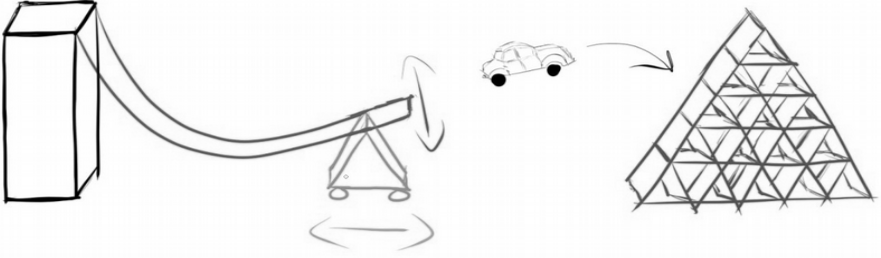
\includegraphics[width=0.7\textwidth]{authors/leybovich-fig1.png}
  \end{center}
  \caption{Схема установки <<Баллистика>>}
  \label{fig:leybovich-fig1}
\end{figure}


Вторая установка (рис. 2) демонстрирует законы сохранения энергии и перехода её из~одного вида в другой (принцип <<домино>>).

Вначале изготавливается каркас для направления движения шара по конструкции. Каркас конструируется из двух горок и двух горизонтально положенных досок. Первая часть установки состоит из стойки, с которой покатится шар, а также горки и доски, по которым шар покатится в мельницу. Мельница собирается из~ножки (используемой как опора) и~подставки (с помощью которой мельница будет держать устойчивое положение). Лопасти мельницы состоят из трёх лёгких перекрещенных дощечек, которые закреплены с помощью шурупа. Шуруп крепится к моторчику, который будет вращать лопасти мельницы. Вторая часть состоит из доски, по которой шар скатывается с мельницы, и горки, по которой шар скатывается вниз к домино, собранному в~виде сердца. Мельница располагается между первой и второй частью установки.\enlargethispage{\baselineskip}

\begin{figure}[h!]
  \begin{center}
    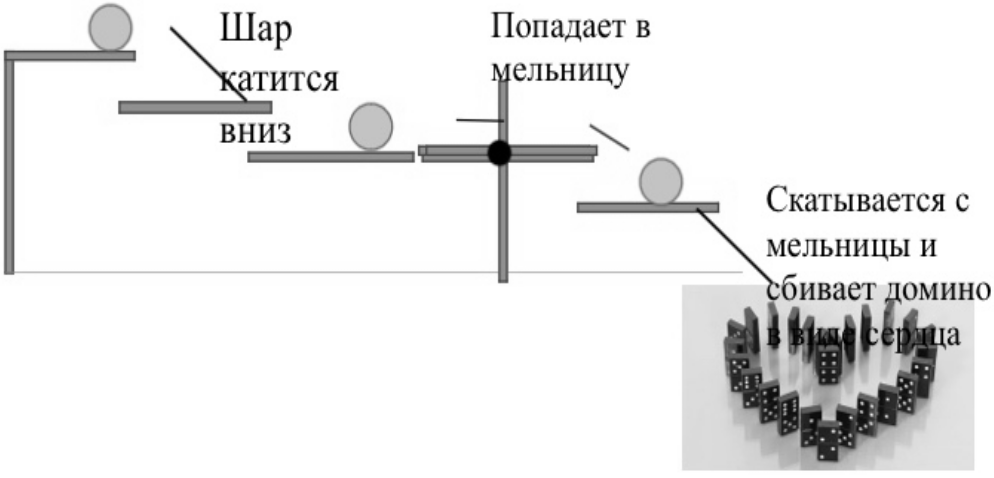
\includegraphics[width=0.7\textwidth]{authors/leybovich-fig2.png}
  \end{center}
  \caption{Схема установки <<Принцип домино>>}
  \label{fig:leybovich-fig2}
\end{figure}


Шар, запущенный по горке, скатывается вниз. Попадая на лопасти вращающейся за~счёт электрического моторчика мельницы он перекатывается на следующую горку, скатываясь по которой сбивает домино, которое сложено в виде сердца. Таким образом, эта~конструкция наглядно демонстрирует законы сохранения в природе.\thispagestyle{empty}

Третья установка имеет более сложную комплектацию и включает множество различных деталей~--- детскую машинку, дорожку для её движения, пластиковые фишки домино, маленькие железные шарики, качели-балансиры, пластиковую трубу и маятник (рис.~3). Её~назначение также заключается в демонстрации законов сохранения и импульса. Для её построения на стул устанавливается небольшая горка. Из семи деревянных дощечек (которые вырезаются из одной большой доски) строятся дорожки. На одной из них, расположенной горизонтально, ставятся фишки домино. В конце дорожки размещается шарик. Другая дощечка располагается под углом (чтобы шарик смог скатиться). Качели-балансиры изготавливаются самостоятельно из простой дощечки и любой опоры. Для установки трубы также используется любая опора (можно выбрать небольшую коробочку или маленький стульчик). По желанию маятник тоже можно изготовить самостоятельно, но его не сложно приобрести и в магазинах.

\begin{figure}[h!]
  \begin{center}
    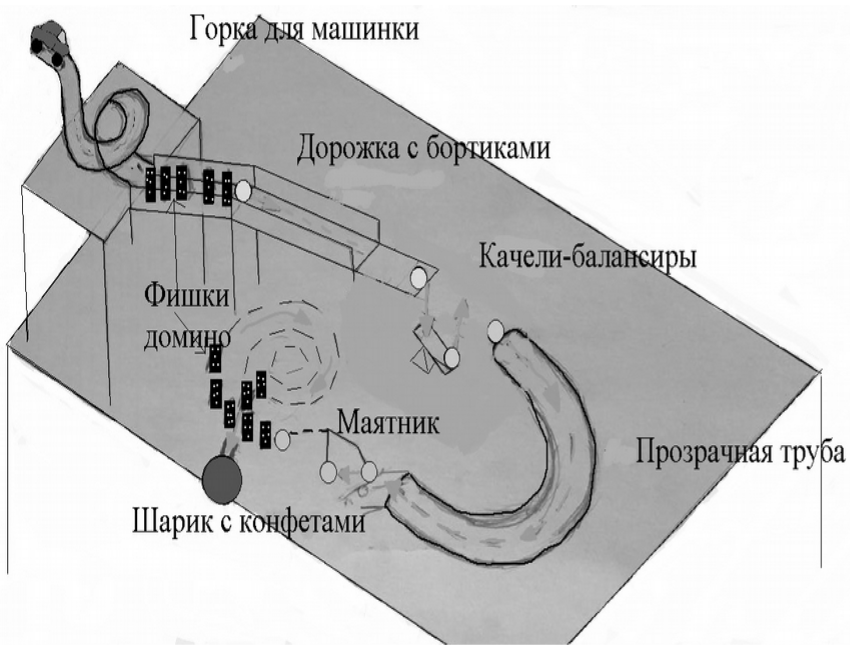
\includegraphics[width=0.9\textwidth]{authors/leybovich-fig3.png}
  \end{center}
  \caption{Схема установки <<Конвейер>>}
  \label{fig:leybovich-fig3}
\end{figure}


Вся работа данной конструкции заключается в том, что предметы, передавая друг другу импульс и энергию, вызывают цепную реакцию движения. На небольшой высоте над поверхностью закрепляется направляющая дорожка, по которой запускается машинка. Скатившись и набрав скорость, она толкает фишки домино, которые в свою очередь приводят в движение шарик.  Шарик падает на качели-балансиры, что позволяет другому шарику подняться под углом вверх и попасть в пластиковую трубу. На выходе из трубы шарик толкает дощечку, удерживающую на небольшой высоте маятник. Вследствие этого маятник начинает колебаться и толкает фишки домино, которые рушатся и складываются в~красивый рисунок. Бонус~--- последняя фишка домино толкает в руки детям шарик с конфетами внутри.

В заключение отметим, что общение разных поколений в ходе конструирования представленных установок позволяет обмениваться им своими знаниями и умениями. А для поколения Z, вступающего в ближайшем будущем в активную профессиональную жизнь, такие занятия позволяют более осознанно принимать решения о выборе своей инженерной специальности. Разработанные нами установки позволяют тренировать и развивать интерес и способности к конструированию и проектированию, что впоследствии сыграет важную роль в освоении новых профессий будущего.

\begin{thebibliography}{99}
\bibitem{}\BibAuthor{}Какие профессии будут востребованы через 5--7 лет [Электрон. ресурс].~--- URL: https://www.iqconsultancy.ru/articles/kakie-professii-budut-vostrebovany-cherez-5-7-let \\(дата обращения: 25.03.2020).

\bibitem{}\BibAuthor{}5 особенностей поколений Z, которые стоит учитывать, чтобы найти с ними общий язык [Электрон. ресурс].~--- URL: https://lifehacker.ru/mif-pokolenie-z (дата обращения: 5.04.2020).
\end{thebibliography}
\thispagestyle{empty}
